\subsection{Region transition probability}

A travel path of a taxi can be simplified as a multi-hop process, in which a hop indicates a load/drop event happened. Seeing that, we define a\emph{ region transition probability} to figure out the probability of the next hop falling in a different region $j$ from the current region $i$. Particularly, two successive events are different. Likewise, the region $i$ and $j$ are recognized by different metrics, that is, drop or load event distribution. It is more reasonable. For an instance, if the taxi is occupied, the next hop event is the drop one. Hence, choosing a target region from a region set divided by drop event distribution is more logical.
%%ÿ���ֲ���ͷһ��Ҫ��&���ţ�����\qquad Ϊ��ո�����

To calculate the region transition probability, the \textbf{region recognition process} should be executed in advance.

Firstly, we divide the area into $100\times 100$ grid, and define cells in it as equation \ref{cell}. Then, we consider region as adjacent cells as equation \ref{region}.

\begin{equation}\label{cell}
\begin{array}{c}
CELL_{x,y}::=\{(lon,lat)|x \le \frac{{lon}}{{len_x}} < x + 1,\\
y \le \frac{{lat}}{{len_y}} < y + 1\}
\end{array}
\end{equation}

\begin{equation}\label{region}
  \begin{array}{r}
REGION_m:: = \{ CEL{L_{x,y}}|\exists CELL_{i,j} \in REGION_m\\
\Rightarrow \|x - i\| \le 1,\|y - j\| \le 1\}
\end{array}
\end{equation}

By clustering cells, two region sets, $\{REGION_m^{load}\}$ and $\{REGION_n^{drop}\}$, can be recognized. The main idea of clustering is to put adjacent cells with event density larger than the event threshold $\eta$ into the same region. To avoid the size of the region become too large or too small, we set a constant $CLUSTERSIZE$ to restrict a region, say $\|REGION_i\|\leq CLUSTERSIZE$ , and only limit the top 200 regions, in which $CELL_{x,y}.events\geq \eta$. After that, the other cells not belong to the top 200 regions, will also be classified into regions, while $\|REGION_j\|\leq CLUSTERSIZE$. Consequently, every cells will be classified into regions and the size of each region is not larger than $CLUSTERSIZE$.

We sort the $100\times 100$ cells by event density in descending order, and begin with the first cell to search its neighbors to ask them whether to join the same region using breadth-first traversal.
The region recognition results for load/drop events are shown in Fig. \ref{figure_region_recognizition}.

In Fig. \ref{figure_region_recognizition}, every colored block presents a region. In addition, the $CLUSTERSIZE=200$, $\eta=121$ for on event and $\eta=141$ for drop event set by the average event density of the top 5000 cells order by its event density. The detailed clustering algorithm is presented in the appendix.

\begin{figure}[!h]
\centering
\subfigure[passenger drop event regions]{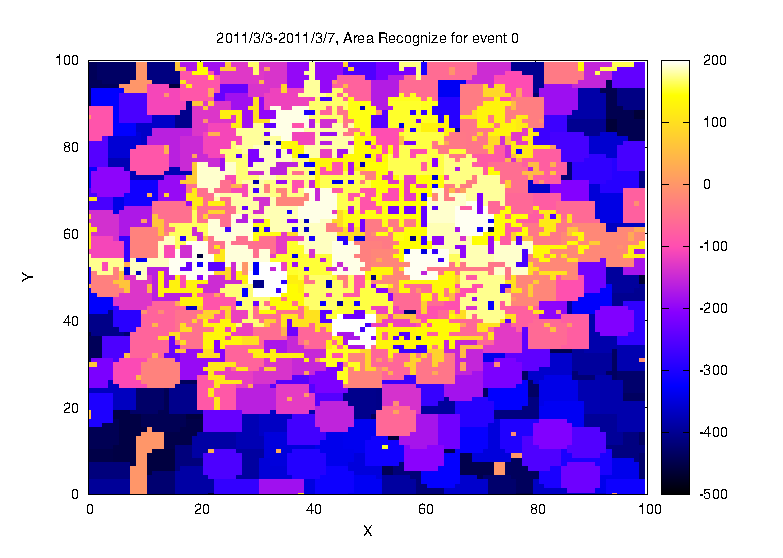
\includegraphics[width=0.23\textwidth]{figures_201103/region/Areas-2011_event0.eps}}
\subfigure[passenger load event regions]{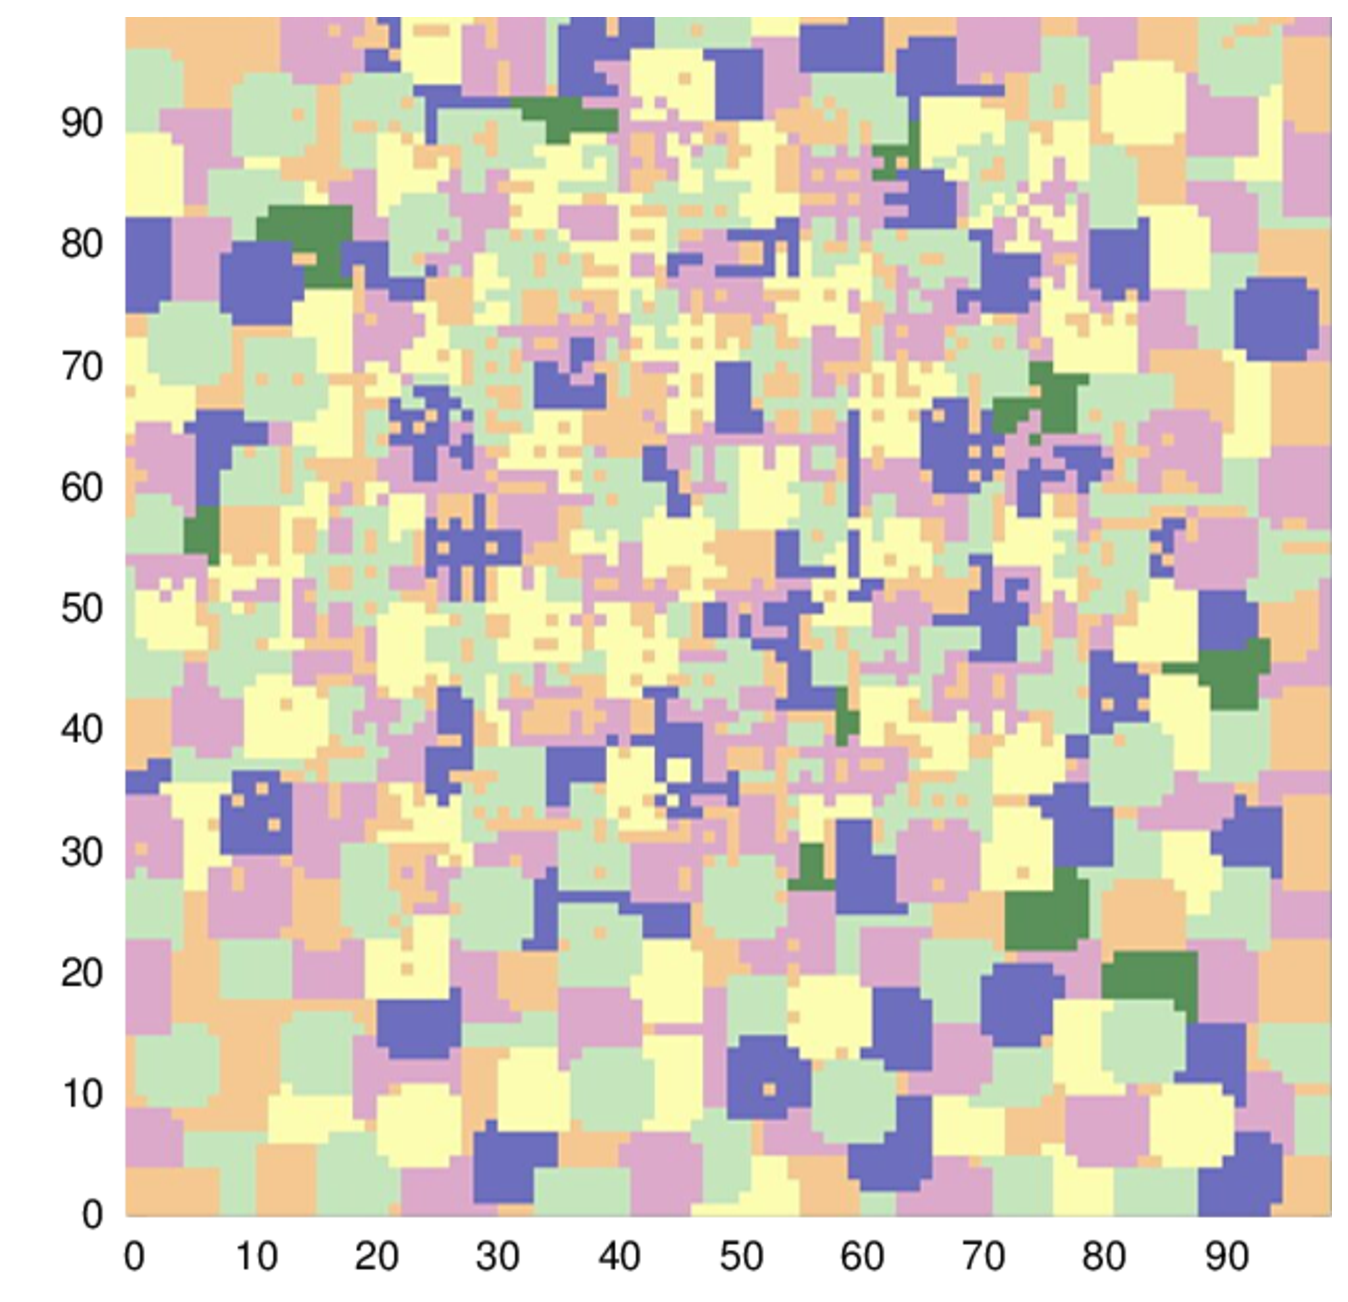
\includegraphics[width=0.23\textwidth]{figures_201103/region/Areas-2011_event1.eps}}
\centering
\caption{Region recognition}\label{figure_region_recognizition}
\end{figure}

\textbf{The calculate process of the region transition probability:} After classifying cells into regions, the transition probability from $REGION_i^{load/drop}$ to $REGION_j^{drop/load}$, denoted as $p_{i\rightarrow j}^{load\rightarrow drop /drop\rightarrow load}$. To substatiate, the calculate process of $p_{i\rightarrow j}^{load\rightarrow drop}$ will be introduced in detail. The records in $REGION_i^{load}$ can be acquired from the data set easily. the record amount is denoted as $\|RECORDS_i^{load}=\{record|record.location\in{REGION_i^{load}\cap record.event=load}\}\|$. For $record \in RECORD_i^{load}$, the next event and location can be easily required. Therefore, the record can be associated with the its next hop information to $(taxiid, location_{current}, event,event_{next},location_{next})$. The $RECORDS_{i\to j}^{load\to drop}=\{record|event=load\cap event_{next}=drop\cap location_{current}\in REGION_i^{load}\cap location_{next}\in REGION_j^{drop}\}$ will be obtained.

\begin{equation}\label{pij}
p_{i \to j}^{load \to drop} = \frac{\|RECORDS_{i\to j}^{load\to drop}\|}{\|RECORDS_i^{load}\|}
\end{equation}


\begin{equation}\label{transition_matrix}
  P^{load\to drop} = (p_{i\to j}^{load\to drop})_{m\times n}
\end{equation}

\begin{equation}\label{transition_matrix}
  P^{drop\to load} = (p_{i\to j}^{drop\to load})_{n\times m}
\end{equation}

%%\begin{equation}\label{equation_taxiset_matrix}
%\textbf{\emph{P^{on\to drop}}}=(p_{i\to j}^{load\to drop})_{m*n}\\
%\textbf{\emph{P^{drop\to load}}}=(p_{i\to j}^{drop\to load})_{n*m}\\
%\end{equatiload}

